\section{Experiments}
\label{sec:exper}


% \OV{Note} from \cite{xie2016edge}: Though popular in image restoration literature, RMSE met-
% ric over disparity are dominated by wrong assignment around
% boundaries.  Thus,  a  disparity  map  with  blurry  boundaries
% might generate better RMSE score than a disparity with a few
% pixels  being  assigned  with  a  wrong  foreground/background
% disparity  value  around  the  boundary.  Therefore,  to  evaluate
% the  accuracy  of  disparity  estima
% tion,  Percent  of  Error  metric
% has been reported as a more fair measurement in stereo related
% fields like stereo matching

In this section, we describe a series of computational experiments
to characterize the performance of several methods for super-resolution with respect to visual 
quality metric. 

We start with an experiment for visual surface quality evaluation based on the results produced by a variety 
of techniques and demonstrate the limitations of RMSE as a visual quality measure. Our second
set of experiments shows the advantages of using a visually-based loss for the modified methods. We further investigate a combined hole-filling/super-resolution method in terms of improvement of visual quality of the surface, using the same loss.

\subsection{Datasets}

We have selected a representative and diverse set of depth images and registered RGB images from 
four datasets most commonly employed in literature on depth super-resolution
\cite{handa:etal:ICRA2014,song2015sun,ferstl2013image,scharstein2014high}. By creating our \emph{SimGeo}
dataset and extracting subsets of images from these datasets, we end up with eight evaluation subsets
(see the table in supplementary materials for a summary of our evaluation set).
% We display samples from these datasets in Fig.~\ref{} and provide 

The \emph{SimGeo} dataset has been created using 
Blender\footnote{Available from \url{http://www.blender.org/}} and consists of simple geometric
shapes without textures as well as with lower- and higher-detailed textures 
(aimed to act as high-frequency and low-frequency intensity components).
Our goal when using \emph{SimGeo} dataset is to benchmark against
a relatively simple set of noise-free depth images, possibly revealing false texture transfer
for RGB-guided upsampling methods.

ICL-NUIM~\cite{handa:etal:ICRA2014} is a photo-realistic synthetic dataset obtained using
advanced rendering techniques, offering ground truth data for quantitative evaluation
of the quality of the final depth-based surface reconstruction. 
Two different scenes (the living room  and the office room scene) are provided.
The dataset offers realistic input images along with synthetic ground truth, 
free from any possible acquisition noise.

%SUN RGB-D~\cite{song2015sun} is a dataset containing $>$10K RGB-D images 
%with dense annotations in both 2D and 3D, for both objects and rooms, 
%captured by four different sensors, including Intel RealSense, 
%Asus Xtion, Kinect v1, and Kinect v2 devices. We select subsets of data
%corresponding to \emph{RealSense}, \emph{Xtion}, and \emph{Kinect v2} devices, named accordingly.
%These datasets correspond to consumer-level RGB-D sensors and provide the most likely
%target application for our depth super-resolution algorithm due
%to the wide availability of the RGB-D data.

%ToFMark~\cite{ferstl2013image} is a challenging real-world benchmarking dataset
%providing real time-of-flight and intensity camera acquisitions together
%with an accurate ground truth measurement using a structured light sensor.
%We include this dataset in our evaluation as we believe it provides
%the most challenging real-world setup available, while featuring a promising time-of-flight sensor.

A widely used dataset Middlebury 2014~\cite{scharstein2014high} consists of complex real-world scenes
captured by an industrial structured light system, with accompanying stereo images.
We extract two subsets from this dataset, which we refer to as \emph{Simple} and \emph{Complex},
with \emph{Complex} dataset consisting of images having significantly finer detailed
surfaces compared to \emph{Simple}. Middlebury datasets are a standard benchmark in depth upsampling methods.
Due to the careful measurement with precise ground truth, they provide the 
best available real-world training and testing data.




\subsection{The evaluation setup}
% \OV{Note} For the samples with invalid values (Middlebury 2014 and SUN-RGBD), using higher order interpolation (bilinear, bicubic) for generation of low-resolution input leads to propagation of invalid values across the image. Because of this, evaluation of super-resolution algorithms on these samples makes little sense.

As discussed in Section~\ref{sec:metrics},
for measuring the visual quality we render the surface, corresponding to super-resolved range-image, lit with directional parallel light source from different locations: behind the camera, straight in the viewing direction, upward, downward-left, and downward-right (Figure~\ref{fig:normals_directions}).
In this section we only demonstrate $\times 4$ upsampling results,
with renders for $\times 2$ and $\times 8$ upsampling factors provided 
in the supplementary material.

% \subsection{The results of our evaluation}
% \OV{Note} Edge-guided \cite{xie2016edge}: 3h on SUN-RGBD -- presumably fails on not hole-filled, so test only on complete images; the results are oversmoothed.

% Sparse-to-dense \cite{mal2018sparse}: the original method, trained on NYUv2 with 200 randomly sampled depth values as input, produces really bad results, probably because our lowest number of samples for their method is ~1000. For more correct comparison, we could retrain Sparse-to-dense for our problems statements.

% Fight ill-posedness \cite{haefner2018fight}: up to 8 minutes per sample
% перенос текстуры даже на семлах, где например их условие кусочно-постоянности альбедо сохраняется
% ну и с границами оно не справляется, тени оно не понимает, так как у них условие бесконечной удаленности плавного источника, которое здесь почти везде нарушено, это объясняет восстановление границы теней как фактуры поверхности
% а почему “муар” на гранях кубика например… могу предположить, что из-за несоответствия их модели даунсемплинга, box-filtering, той модели, в которой получен лоу рез сдесь — nn.как ни странно, при получении лоу-рез с помощью сглаживающих моделей даунсеплинга результат не лучше
% еще одно предположение — почему их метод хреново сработал на наших данных: у них есть веса разных членов энергетического функционала, которые они подобрали так, чтобы минимизировать лосс на их данных.может для наших данных оптимальные значения параметров — другие
% ну и еще одно предположение, что все может ломаться суммарно из-за несоответствия их прайорам там и сям
% -- тут видно, как на акуле белый цвет переносится в гладкую оверхность, а серый в шероховатую, как будто
% я думаю что здесь просто вход совсем плохой, поэтому и выход плохой
% у них вроде нет никакой явной регуляризации на шумность измерений по глубине, а тут снимок с реальной тоф-камеры, очень шумный
% -- Я бы так сказал - иногда rgb дает неправильный guidance
%   Во введении к статье minimum spanning trees об этом много написано
%   Они там типа с этим борются
% ну и да, текстура может быть воспринята как фактура


% \textsl{Notes} MSG-net, bicubic downsampling, Nans -> destroys the upsampling (huge holes) 


\begin{table*}[t]
\centering
\begin{tabular}{lccccccccc}
\toprule
 & \multicolumn{4}{c}{Sphere and cylinder $\times 4$} && \multicolumn{4}{c}{Lucy $\times 4$}\\
        \cmidrule{2-5} \cmidrule{7-10}\\
Method          & RMSE & SURF & DSSIM & LPIPS && RMSE & SURF & DSSIM & LPIPS \\
\midrule
Bicubic & 0.057 & 0.067 & 0.094 & 0.312     && 0.072 & 0.137 & 0.176 & 0.391 \\
SRfS & 0.059 & 0.088 & 0.215 & 0.643        && 0.082 & 0.297 & 0.405 & 0.777 \\
PDN & 0.157 & 0.052 & 0.130 & 0.338         && 0.173 & 0.143 & 0.261 & 0.435 \\
Edge-Guided & 0.056 & 0.032 & 0.118 & 0.434 && 0.069 & 0.102 & 0.222 & 0.497 \\
MSG & 0.040 & 0.063 & 0.143 & 0.480         && 0.054 & 0.135 & 0.224 & 0.482 \\
DIP-MSE & 0.049 & 0.149 & 0.427 & 0.909  && 0.053 & 0.249 & 0.413 & 0.608 \\
MSG-SURF & 0.100 & 0.022 & 0.038 & 0.172   && 0.074 & 0.056 & 0.102 & 0.250 \\
DIP-SURF & 0.035 & 0.037 & 0.104 & 0.501      && 0.044 & 0.099 & 0.209 & 0.435  \\
\midrule
 & \multicolumn{4}{c}{Livingroom $\times 4$} && \multicolumn{4}{c}{Recycle $\times 4$} \\
        \cmidrule{2-5} \cmidrule{7-10}\\
Method & RMSE & SURF & DSSIM & LPIPS     && RMSE & SURF & DSSIM & LPIPS \\
\midrule
Bicubic & 0.028 & 0.072 & 0.211 & 0.536     && 0.0210 & 0.1309   &   0.3690    &   0.5623 \\
SRfS & 0.039 & 0.188 & 0.353 & 0.608        && 0.0471 & 0.2866   &   0.4056    &   0.6821 \\
PDN & 0.151 & 0.100 & 0.256 & 0.685         && 0.0912 & 0.1775   &   0.3713    &   0.5941 \\
Edge-Guided & 0.036 & 0.094 & 0.251 & 0.735 &&  --    &  --      &    --       &    -- \\
MSG & 0.021 & 0.078 & 0.247 & 0.466         && 0.0974 & 0.3019   &   0.4178    &   0.6752 \\
DIP-MSE & 0.030 & 0.257 & 0.401 & 0.632  && 0.0291 & 0.3660   &   0.4664    &   0.6271 \\
MSG-SURF & 0.068 & 0.039 & 0.176 & 0.526   && 0.0522 & 0.1526   &   0.3703    &   0.5864 \\
DIP-SURF & 0.022 & 0.075 & 0.283 & 0.380      && 0.0204 & 0.1504   &   0.3865    &   0.4993 \\
\bottomrule
\end{tabular}
\caption{Quantitative comparison. Lower values are better for all metrics; RMSE is in meters.}
\label{tab:results}
\vspace{-3pt}
\end{table*}




\subsection{Is RMSE correlated with the perceived quality of~the~3D~surface?}
\label{subsec:is_rmse_correlated}
Our first experimental evaluation demonstrates that
RMSE-related metrics are not well-correlated with visual surface quality. 
We run all  methods (see section~\ref{sec:methods}) to compute estimates $\hiresdepthest_{ij}$ ($i$ indexes methods and $j$ indexes sample depth maps)
of high-resolution depth maps given their low-resolution counterparts
and corresponding high-resolution RGB images (where applicable). We use the box downsampling to compute the low-resolution depth maps where it is necessary. Using the metrics discussed above (see section~\ref{sec:metrics}), we compute 
distances $e_{ijk} = \mathcal{E}_k(\hiresdepth, \hiresdepthest_{ij})$ (where $k$ indexes metrics).
We present a visualization of the correlation between RMSE and visual metrics,
as well as correlation between several visual metrics,
in Fig.~\ref{fig:is_rmse_scatterplots}.  Each point in the plot corresponds to a test image.
Note that our visually-based SURF metric correlate with the perceptual losses significantly better than RMSE, although somewhat 
worse than SSIM correlates with LPIPS.
In Fig.~\ref{fig:is_rmse_visual} we present a subset of the qualitative
results and refer to supplementary material for more visualizations. 

\subsection{Super-resolution results using a~visually-based metric proxy}
\label{subsec:visually_based_proxy}
In the following experiment we evaluate our novel visually-based loss function ~\eqref{eq:our_visual_metric}. %Therefore we train one of the state-of-the-art CNN models, MSG-Net, only modifying the loss-function and keeping the rest of the training setup with accordance to the original work. 
We train MSG-Net on patches, collected from both real-world Middlebury and synthetic MPI Sintel \cite{Butler:ECCV:2012} datasets.

Both the qualitative (Fig.~\ref{fig:is_rmse_visual}) and quantitative (Table~\ref{tab:results}) evaluation according to the perceptual metrics suggest that using visually-based loss function for training leads to significant improvement of visual surface quality. Note that our loss-function not only improves the visual quality of the surface, but also helps to super-resolve fine details, see Fig.~\ref{fig:flower_fine}.

\subsection{Super-resolution and inpainting results using a~zero-shot architecture}
\label{subsec:dip_experiments}
We observe that due to missing values occurring in the input low-resolution depth maps certain methods (\eg, MSG-Net) output large holes in the upsampled result (see the 3rd row of Fig.~\ref{fig:is_rmse_visual}). 
Using the modified deep image prior method, we demonstrate that usage of visually-based loss function~\eqref{eq:our_visual_metric} significantly improves visual quality of the produced surface, see Fig.~\ref{fig:dip_recycle} and Fig.~\ref{tab:results}.  Additional results can be found in the supplementary document.

\begin{figure}[hb!]
\begin{center}
\includegraphics[width=2.8in]{Figures/depth_superresolution/scatter_plots.png}
\end{center}
   \caption{Scatter plots for different metrics used in our evaluation. The top row represent the correlation between visually-based metrics and RMSE. The bottom row represent the correlation between visual metrics.
   }
\label{fig:is_rmse_scatterplots}
\end{figure}

\begin{figure*}[p!]
\begin{center}
% \fbox{\rule{0pt}{4cm} \rule{0.95\linewidth}{0pt}}
% 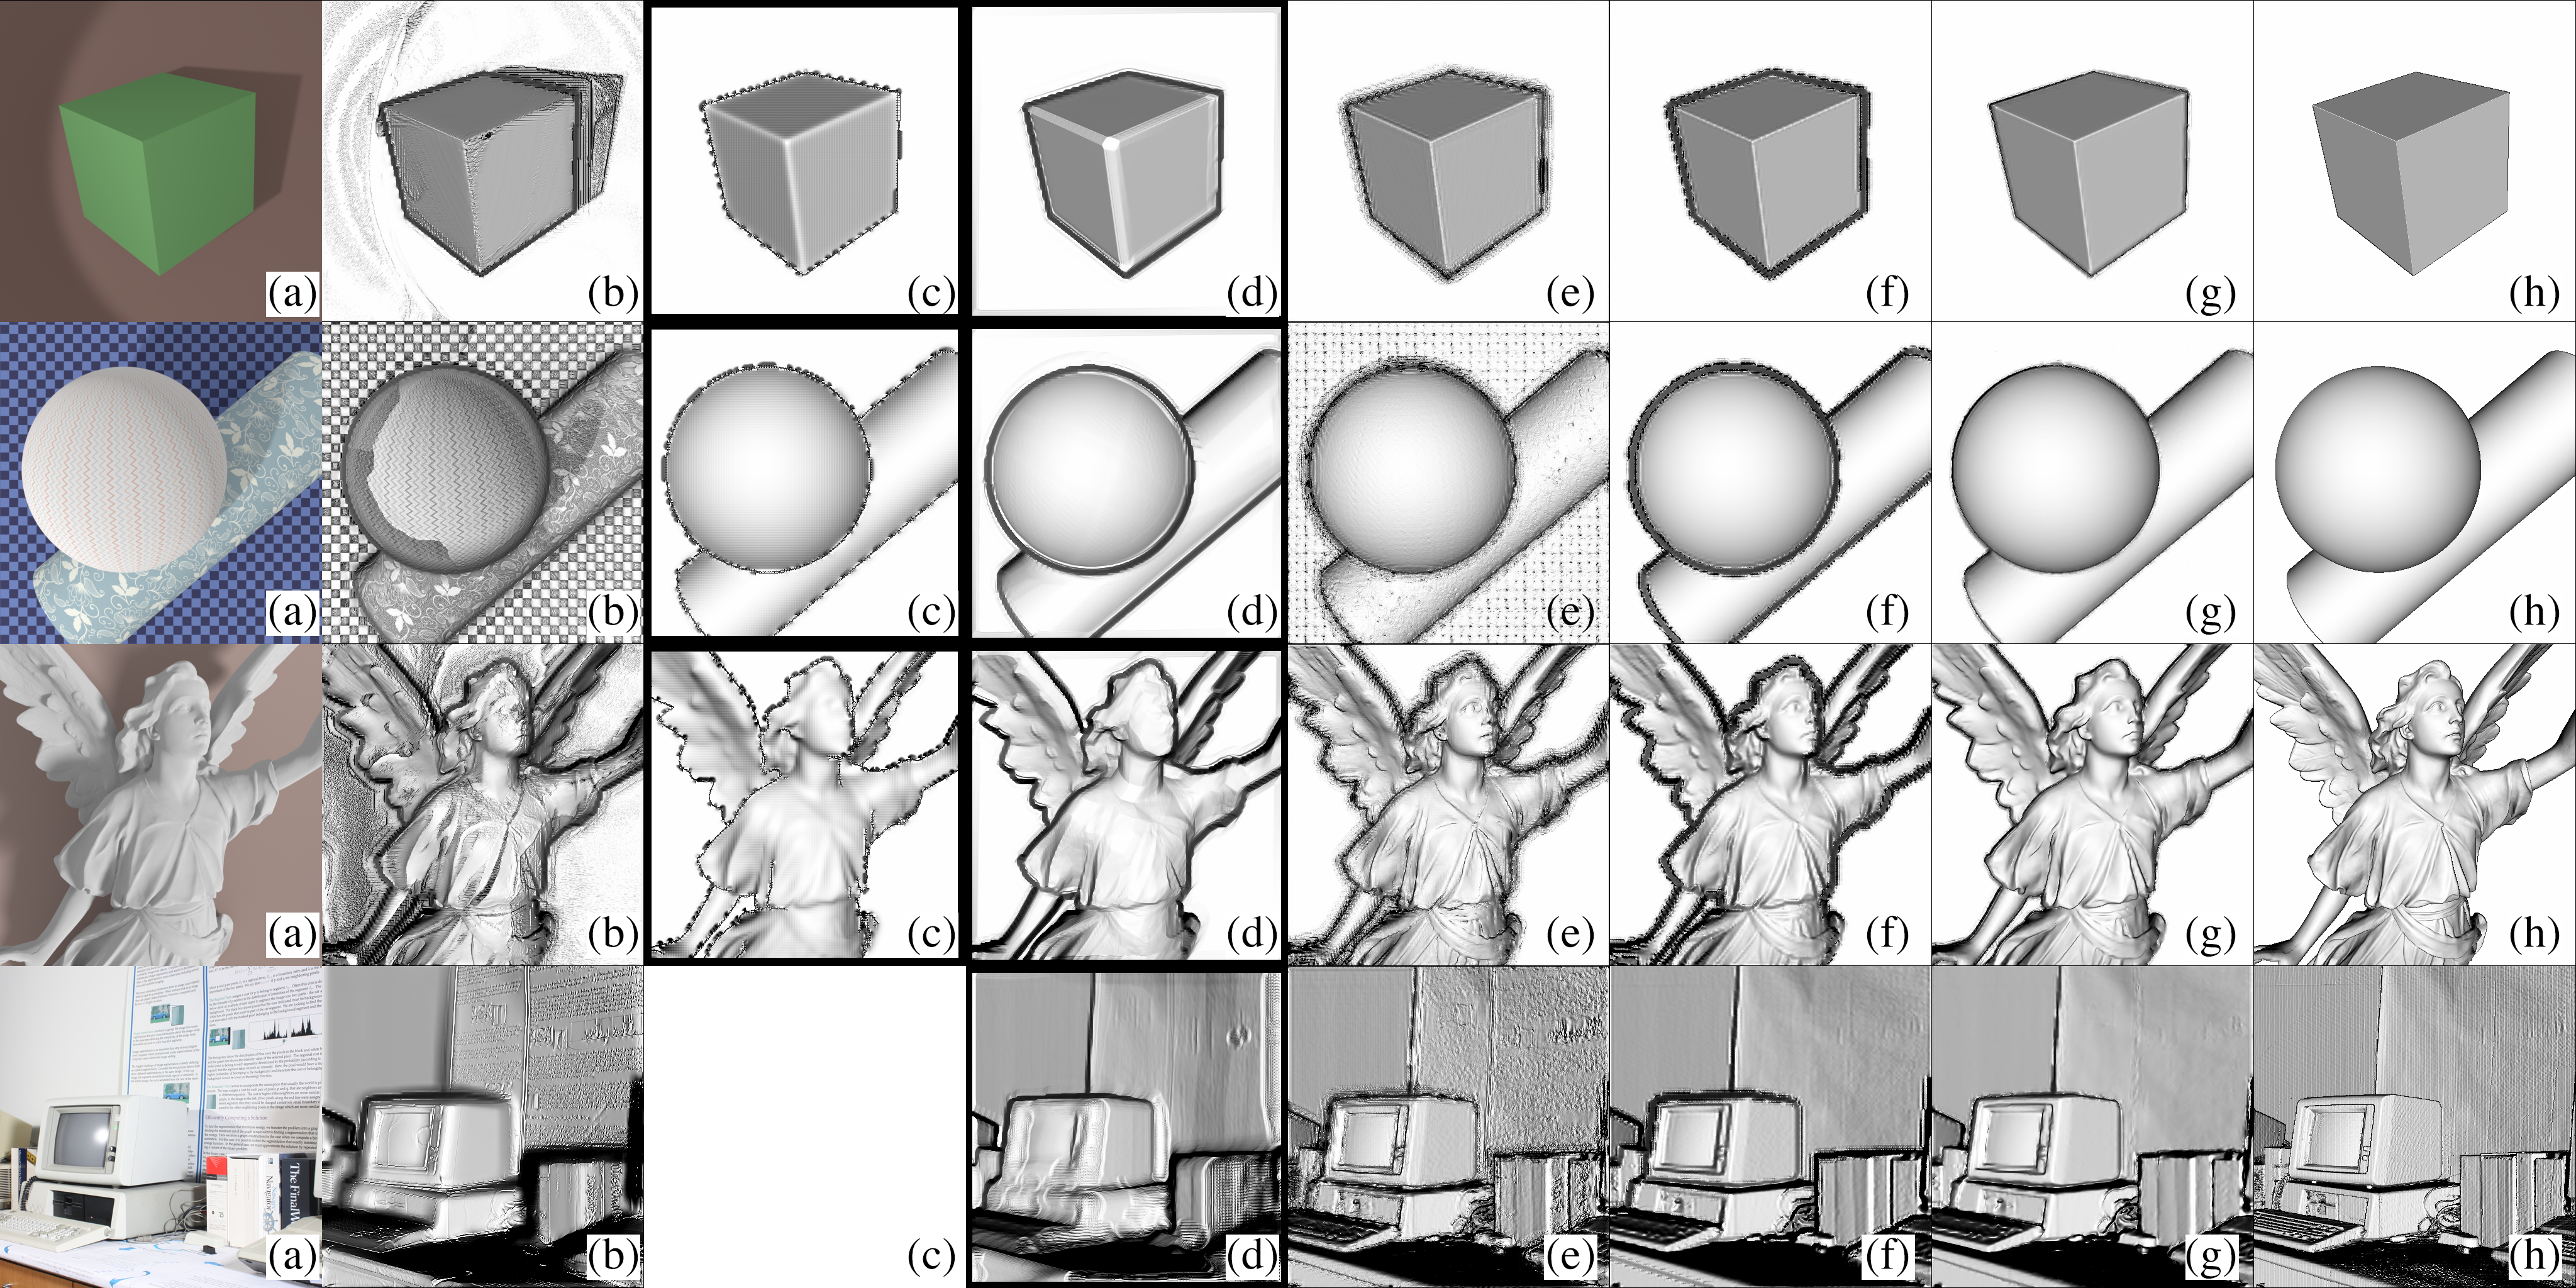
\includegraphics[width=0.995\linewidth]{Figures/depth_superresolution/experiment1.png}
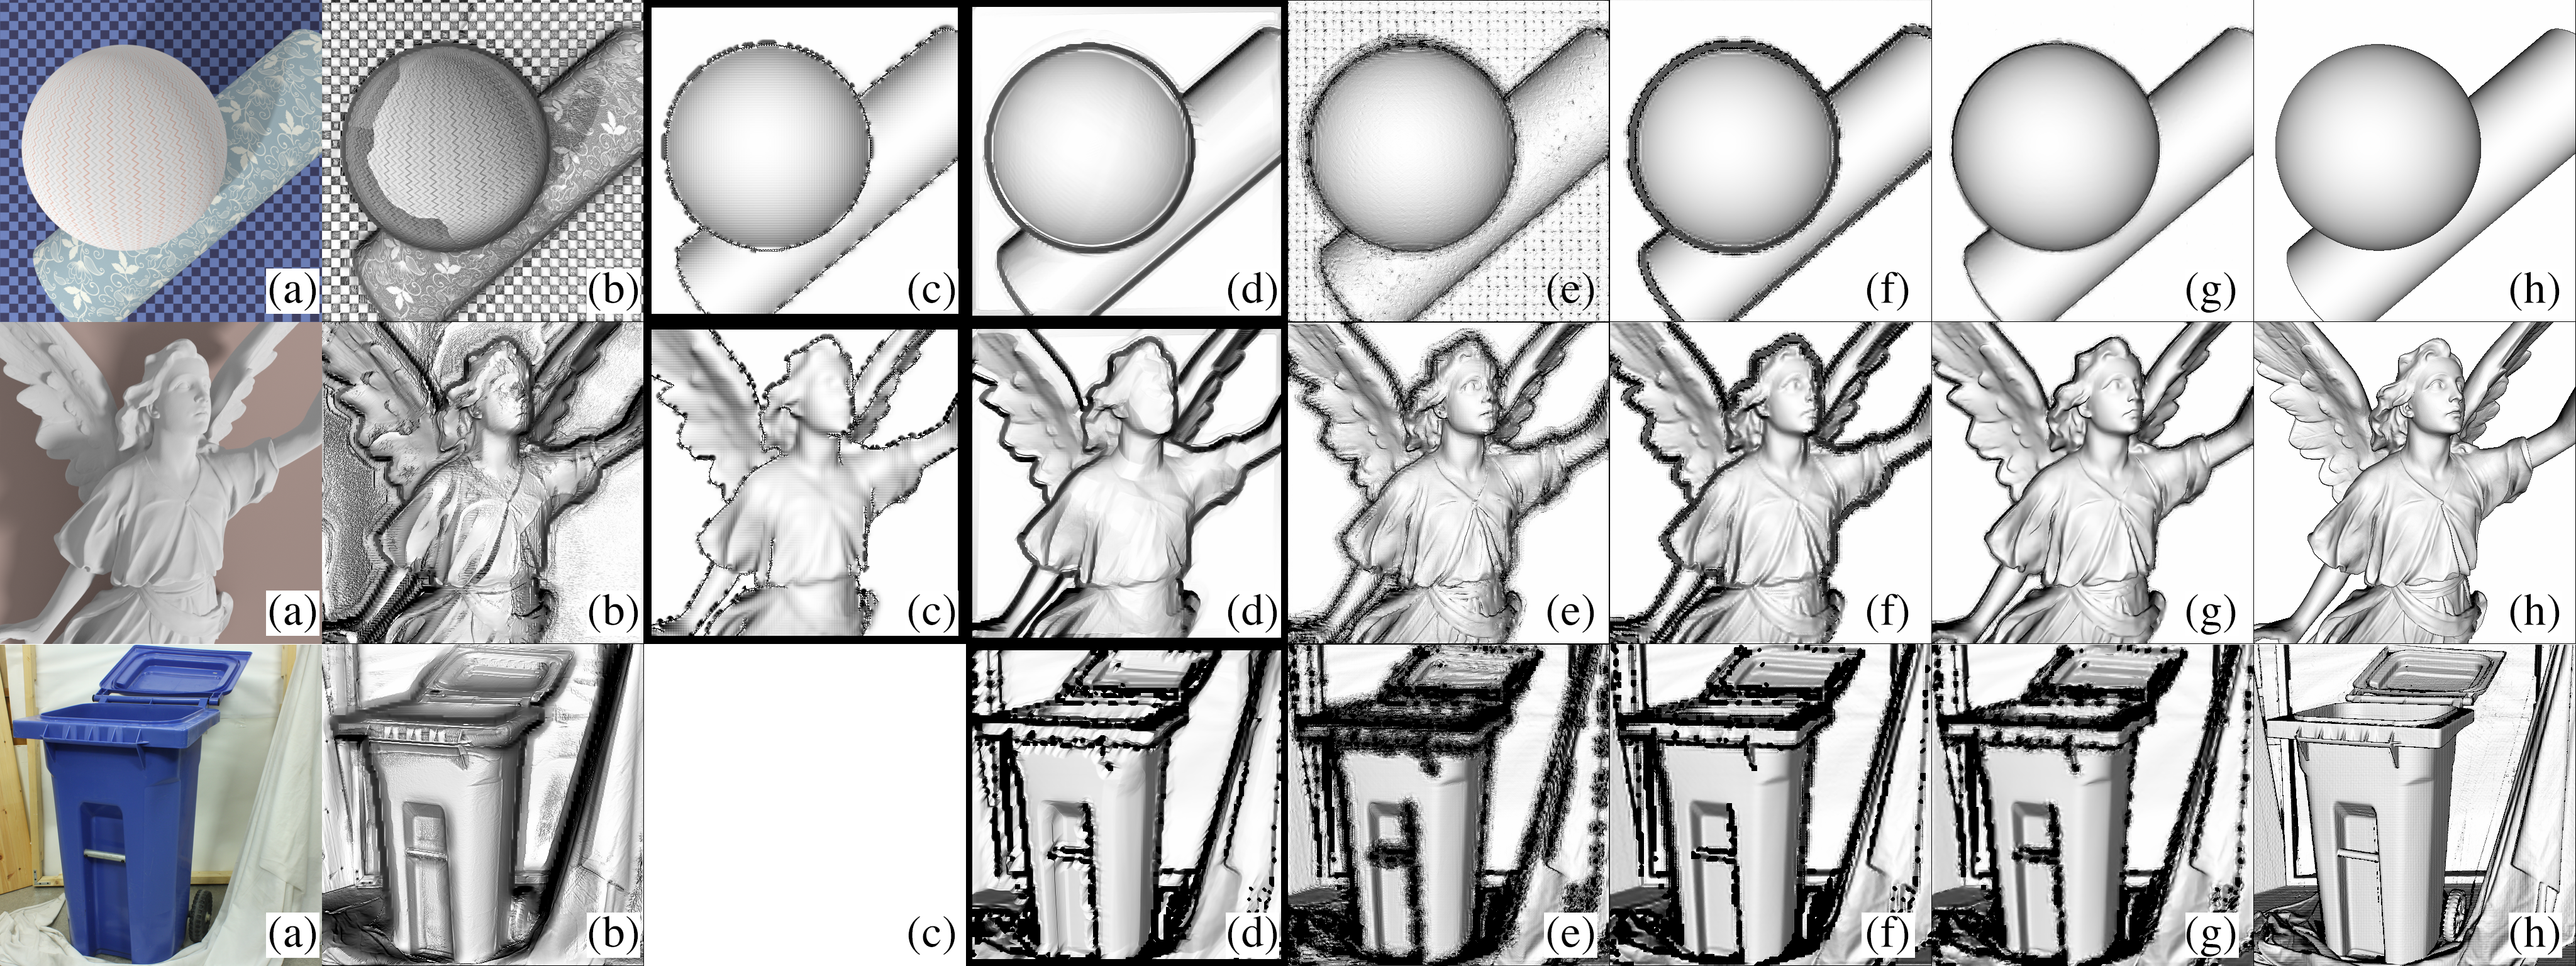
\includegraphics[width=0.995\linewidth]{Figures/depth_superresolution/experiment1.slim.png}
\end{center}
   \caption{A visual comparison of the results obtained or set of methods, visualized using simple single-source lighting. a) RGB, b) SRfS \cite{haefner2018fight}, c) Edge-Guided \cite{xie2016edge} (the method \cite{xie2016edge} failed completely on this sample), d) PDN \cite{riegler2016deep}, e) MSG \cite{hui2016depth}, f) Bicubic, g) MSG-SURF, h) GT.
   }
\label{fig:is_rmse_visual}
\end{figure*}

\begin{figure*}[p!]
\begin{center}
% \fbox{\rule{0pt}{4cm} \rule{0.95\linewidth}{0pt}}
% 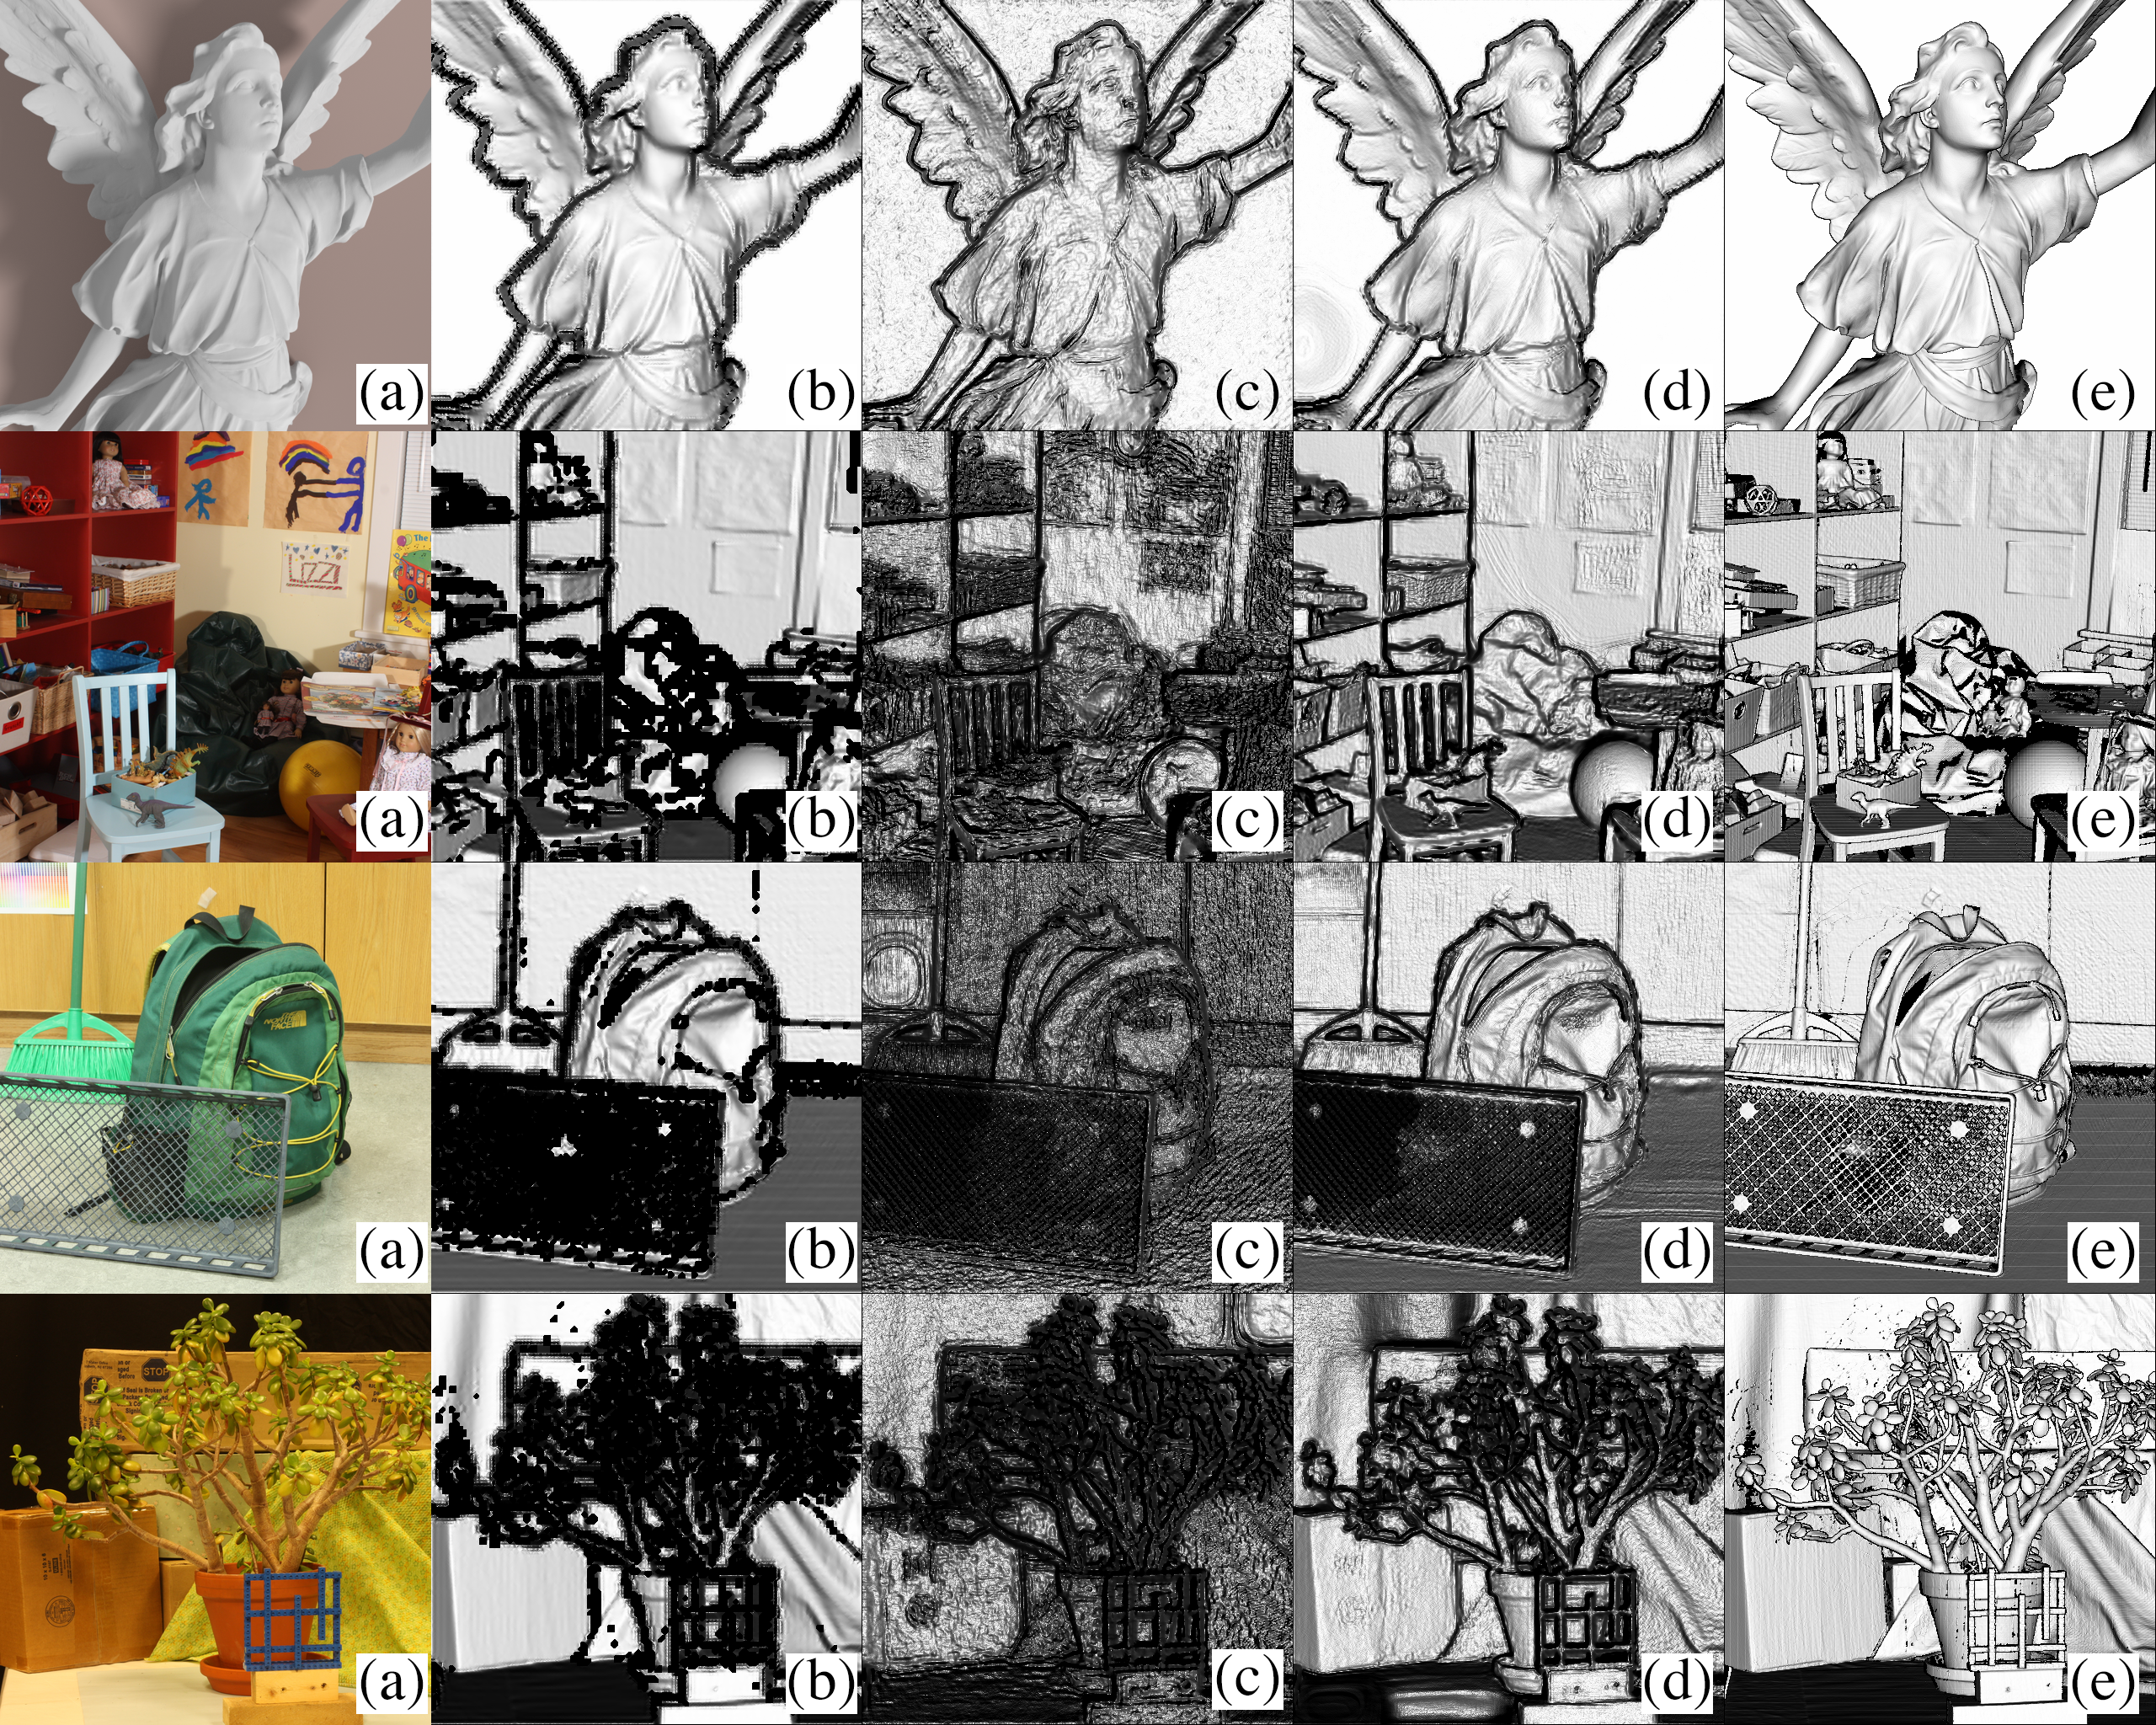
\includegraphics[width=0.995\linewidth]{Figures/depth_superresolution/experiment3.png}
\includegraphics[width=0.995\linewidth]{Figures/depth_superresolution/experiment3.slim.png}
\end{center}
   \caption{The visual comparison of the results, obtained with \cite{Ulyanov_2018_CVPR} using MSE loss -- a) and c), and our loss -- b) and f).}
\label{fig:dip_recycle}
\end{figure*}

\begin{figure*}[p!]
\begin{center}
% \fbox{\rule{0pt}{4cm} \rule{0.95\linewidth}{0pt}}
\includegraphics[width=0.995\linewidth]{Figures/depth_superresolution/experiment1.a.png}
\end{center}
   \caption{4x super-resolution for the "Living Room" sample from ICL-NUIM dataset. a) RGB, b) SRfS \cite{haefner2018fight}, c) Edge-Guided \cite{xie2016edge}, d) PDN \cite{riegler2016deep}, e) MSG \cite{hui2016depth}, f) Bicubic, g) MSG-SURF, h) GT.}
\label{fig:flower_fine}
\end{figure*}